%------------------------------------------------
\section{Kết luận \& hướng phát triển}
\SectionIntro{Phần 4: Kết luận \& hướng phát triển}{Tổng kết kết quả đạt được và định hướng nghiên cứu tương lai.}
%------------------------------------------------
% Định nghĩa màu sắc giống trong ảnh
\definecolor{myRed}{HTML}{FF3B30}   % Màu đỏ đậm cho số %
\definecolor{myBlue}{HTML}{006994}  % Màu xanh cho tiêu đề bảng
\definecolor{myTextBlue}{HTML}{2E86C1} % Màu xanh nhạt cho nội dung
\definecolor{highlightYellow}{RGB}{255, 222, 89}
% Định nghĩa mã màu tương ứng với ảnh
\definecolor{orangeTitle}{RGB}{235, 131, 10}
\definecolor{orangeBg}{RGB}{255, 251, 240}
\definecolor{blueTitle}{RGB}{30, 100, 180}
\definecolor{blueBg}{RGB}{242, 247, 252}
% Định nghĩa mã màu xanh (Blue) tương ứng với ảnh
\definecolor{mainblue}{RGB}{28, 117, 188}
\definecolor{bgblue}{RGB}{245, 249, 253}
% Cấu hình hộp tcolorbox cho từng cột
\tcbset{
    limitationbox/.style={
        colback=bgblue,
        colframe=mainblue,
        boxrule=0pt,
        leftrule=0pt, % Tạo đường kẻ xanh bên trái
        arc=5pt,
        sharp corners=northwest,
        sharp corners=southwest,
        height=5.5cm, % Cố định chiều cao để các hộp bằng nhau
        valign=top,
        halign=center,
        fontupper=\small,
        boxsep=5pt,
        left=8pt, right=8pt, top=10pt
    }
}


\begin{frame} 
    \frametitle{\textbf{KẾT QUẢ THỰC NGHIỆM}}
    
    \begin{columns}[c] % Căn giữa theo chiều dọc
        % --- CỘT TRÁI: SỐ TO ---
        \begin{column}{0.4\textwidth}
            \centering
            % Giữ nguyên font to
            {\fontsize{40}{45}\selectfont \textbf{\textcolor{myRed}{96.45\%}}}
            
            \vspace{0.2em}
            {\Large \textcolor{myTextBlue}{Accuracy}}
        \end{column}
        
        % --- CỘT PHẢI: BẢNG CHI TIẾT ---
        \begin{column}{0.6\textwidth}
            \centering
            \renewcommand{\arraystretch}{1.2} 
            \setlength{\tabcolsep}{8pt} % Thu nhỏ khoảng cách cột cho vừa khung
            
            \begin{tabular}{l r}
                \textcolor{myBlue}{\textbf{Chỉ số}} & \textcolor{myBlue}{\textbf{Giá trị}} \\
                \arrayrulecolor{gray!40}\midrule
                
                \textcolor{myTextBlue}{Accuracy (\%)} & \textcolor{myTextBlue}{96.45} \\
                \textcolor{myTextBlue}{Precision}     & \textcolor{myTextBlue}{0.9646} \\
                \textcolor{myTextBlue}{Recall}        & \textcolor{myTextBlue}{0.9645} \\
                \textcolor{myTextBlue}{F1-Score}      & \textcolor{myTextBlue}{0.9645} \\
                \arrayrulecolor{gray!40}\midrule
                
                \textcolor{myTextBlue}{Số tham số (M)} & \textcolor{myTextBlue}{7.70} \\
                \textcolor{myTextBlue}{Time (phút)} & \textcolor{myTextBlue}{33.95} \\
                
            \end{tabular}
        \end{column}
    \end{columns}
\end{frame}

\begin{frame}
    \frametitle{KẾT QUẢ PHÂN LOẠI}

    \vspace{0.3cm}
    \begin{columns}[T] 
        % --- CỘT TRÁI: HÌNH ẢNH MA TRẬN ---
        \begin{column}{0.48\textwidth}
            \centering
            \includegraphics[width=\linewidth, keepaspectratio]{images/TongKet/MaTran.png}
        \end{column}

        % --- CỘT PHẢI: CÁC Ô THÔNG TIN ---
        \begin{column}{0.50\textwidth}
            \scriptsize 
            
            % Hàng 1
            \begin{columns}[T]
                \begin{column}{0.49\textwidth}
                    \begin{tcolorbox}[colback=green!10, colframe=green!60!black, 
                        title=\textbf{297 (TN)}, % Rút gọn tiêu đề để tránh tràn hàng
                        boxrule=0.5mm, arc=1.5mm, left=1pt, right=1pt, top=2pt, bottom=2pt,
                        halign=flush left] % Sửa lỗi Underfull hbox
                        Dự đoán đúng normal.
                    \end{tcolorbox}
                \end{column}
                
                \begin{column}{0.49\textwidth}
                    \begin{tcolorbox}[colback=green!10, colframe=green!60!black, 
                        title=\textbf{273 (TP)}, 
                        boxrule=0.5mm, arc=1.5mm, left=1pt, right=1pt, top=2pt, bottom=2pt,
                        halign=flush left]
                        Dự đoán đúng defect.
                    \end{tcolorbox}
                \end{column}
            \end{columns}
            
            \vspace{0.1cm}

            % Hàng 2
            \begin{columns}[T]
                \begin{column}{0.49\textwidth}
                    \begin{tcolorbox}[colback=red!10, colframe=red!60!black, 
                        title=\textbf{13 (FN)}, 
                        boxrule=0.5mm, arc=1.5mm, left=1pt, right=1pt, top=2pt, bottom=2pt,
                        halign=flush left]
                        Bỏ sót lỗi.
                    \end{tcolorbox}
                \end{column}
                
                \begin{column}{0.49\textwidth}
                    \begin{tcolorbox}[colback=orange!10, colframe=orange!60!black, 
                        title=\textbf{8 (FP)}, 
                        boxrule=0.5mm, arc=1.5mm, left=1pt, right=1pt, top=2pt, bottom=2pt,
                        halign=flush left]
                        Báo nhầm.
                    \end{tcolorbox}
                \end{column}
            \end{columns}
            
        \end{column}
    \end{columns}

    \vspace{-0.2cm}
    \centering
    \small \textbf{Kết luận:} Mô hình cân bằng tốt giữa việc phát hiện lỗi và hạn chế báo động giả.
\end{frame}

\begin{frame}
\label{Bieudo}
	\frametitle{BIỂU ĐỔ QUÁ TRÌNH HUẤN LUYỆN}
	\begin{center}
		\includegraphics[width=1.0\textwidth]{images/TongKet/bieudo.png}
	\end{center}
\end{frame}

\begin{frame}
\label{Test}
	\frametitle{TẬP KIỂM THỬ NGẪU NHIÊN}
	\begin{center}
		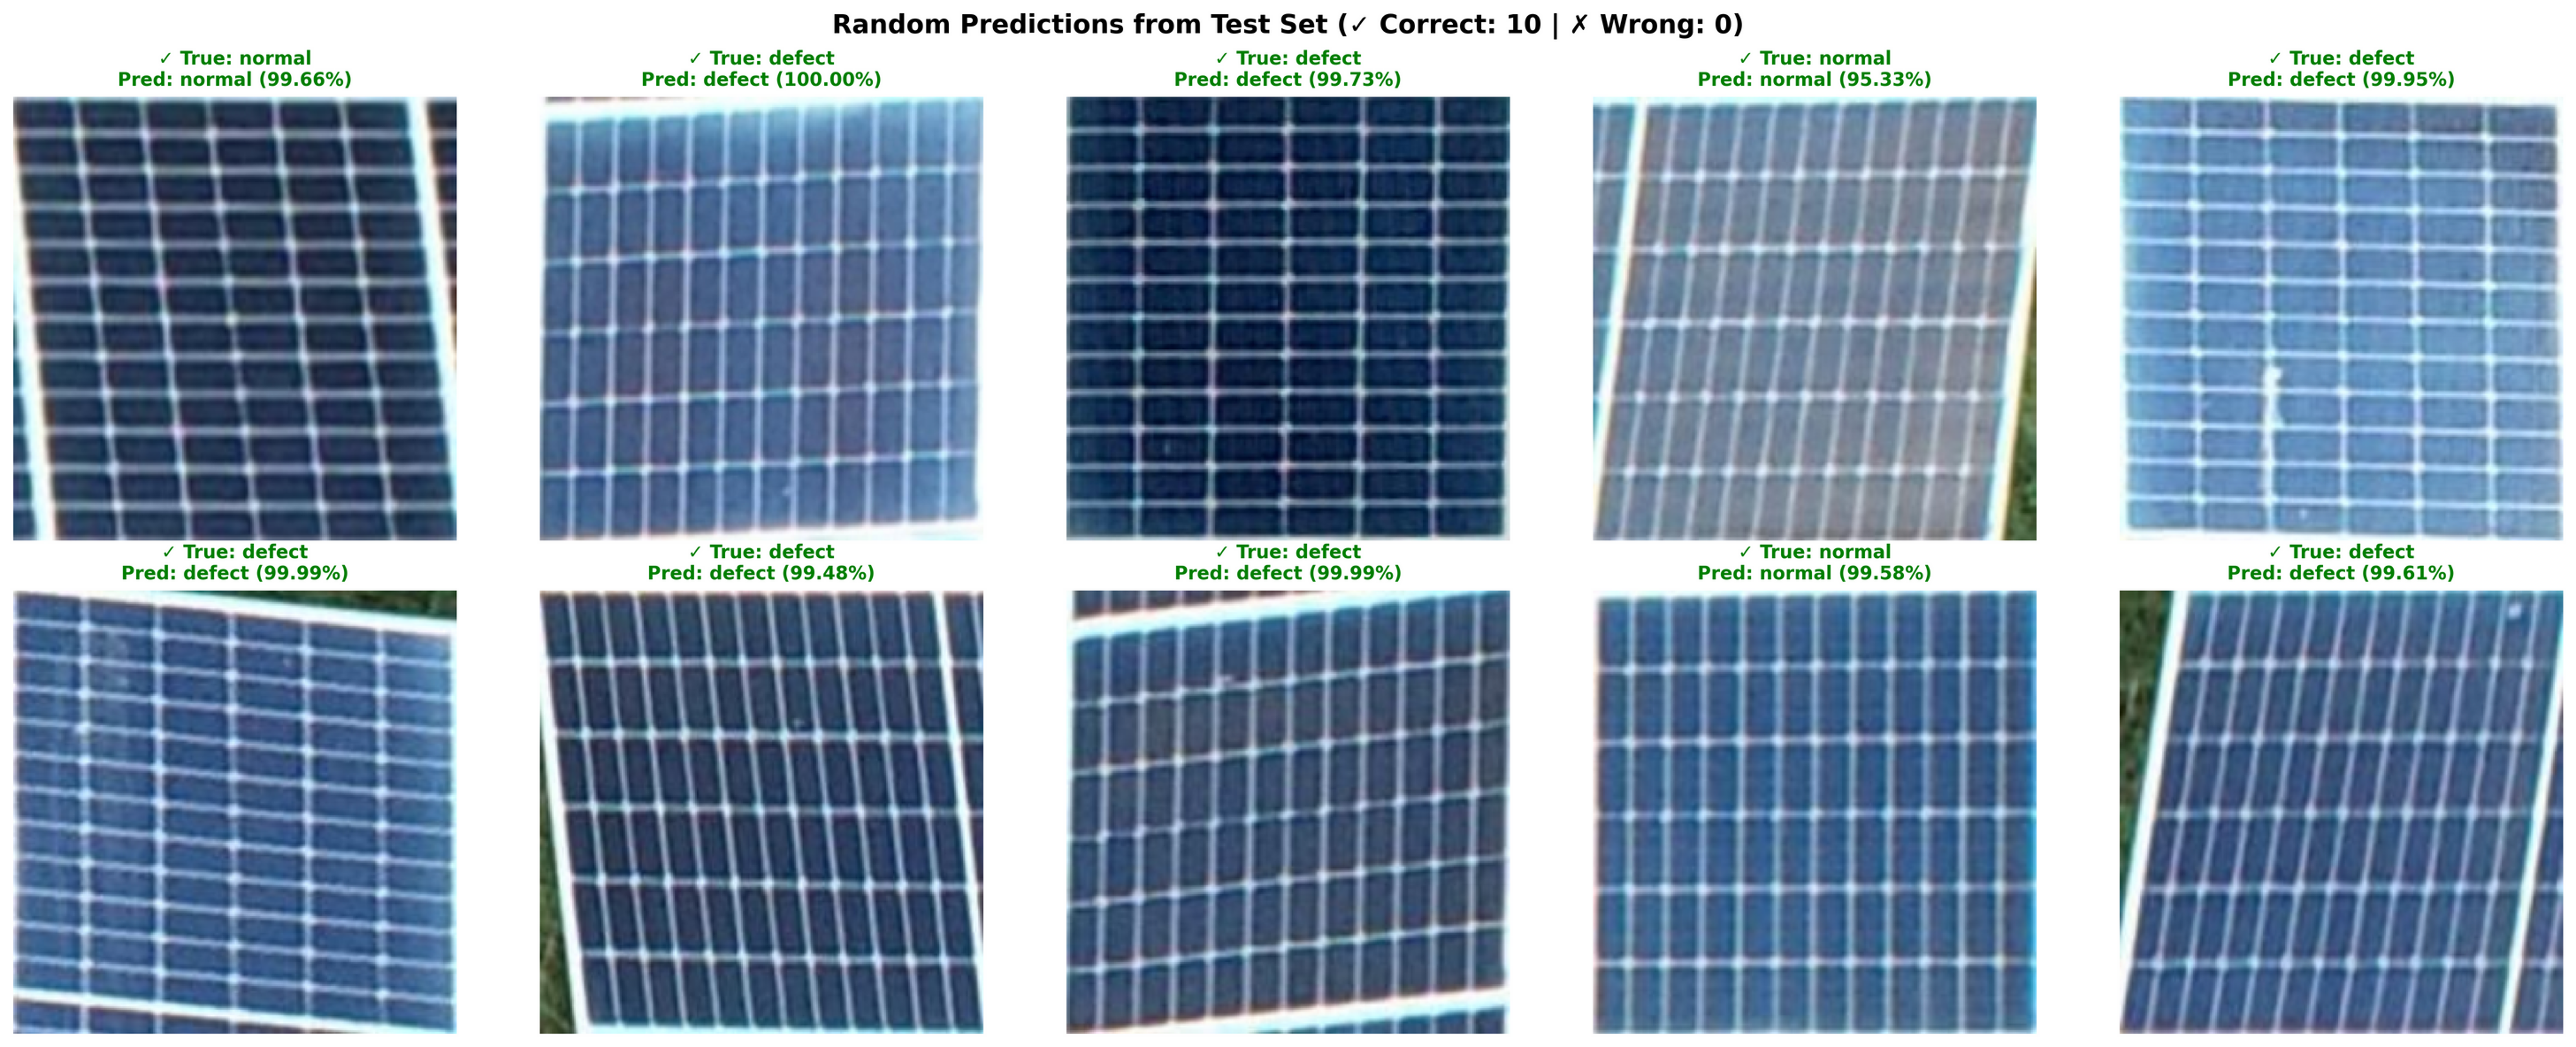
\includegraphics[width=1.0\textwidth]{images/TongKet/test.png}
	\end{center}
\end{frame}

\begin{frame}
\label{Demo1}
	\frametitle{DEMO KẾT QUẢ NHẬN DẠNG}
	\begin{center}
		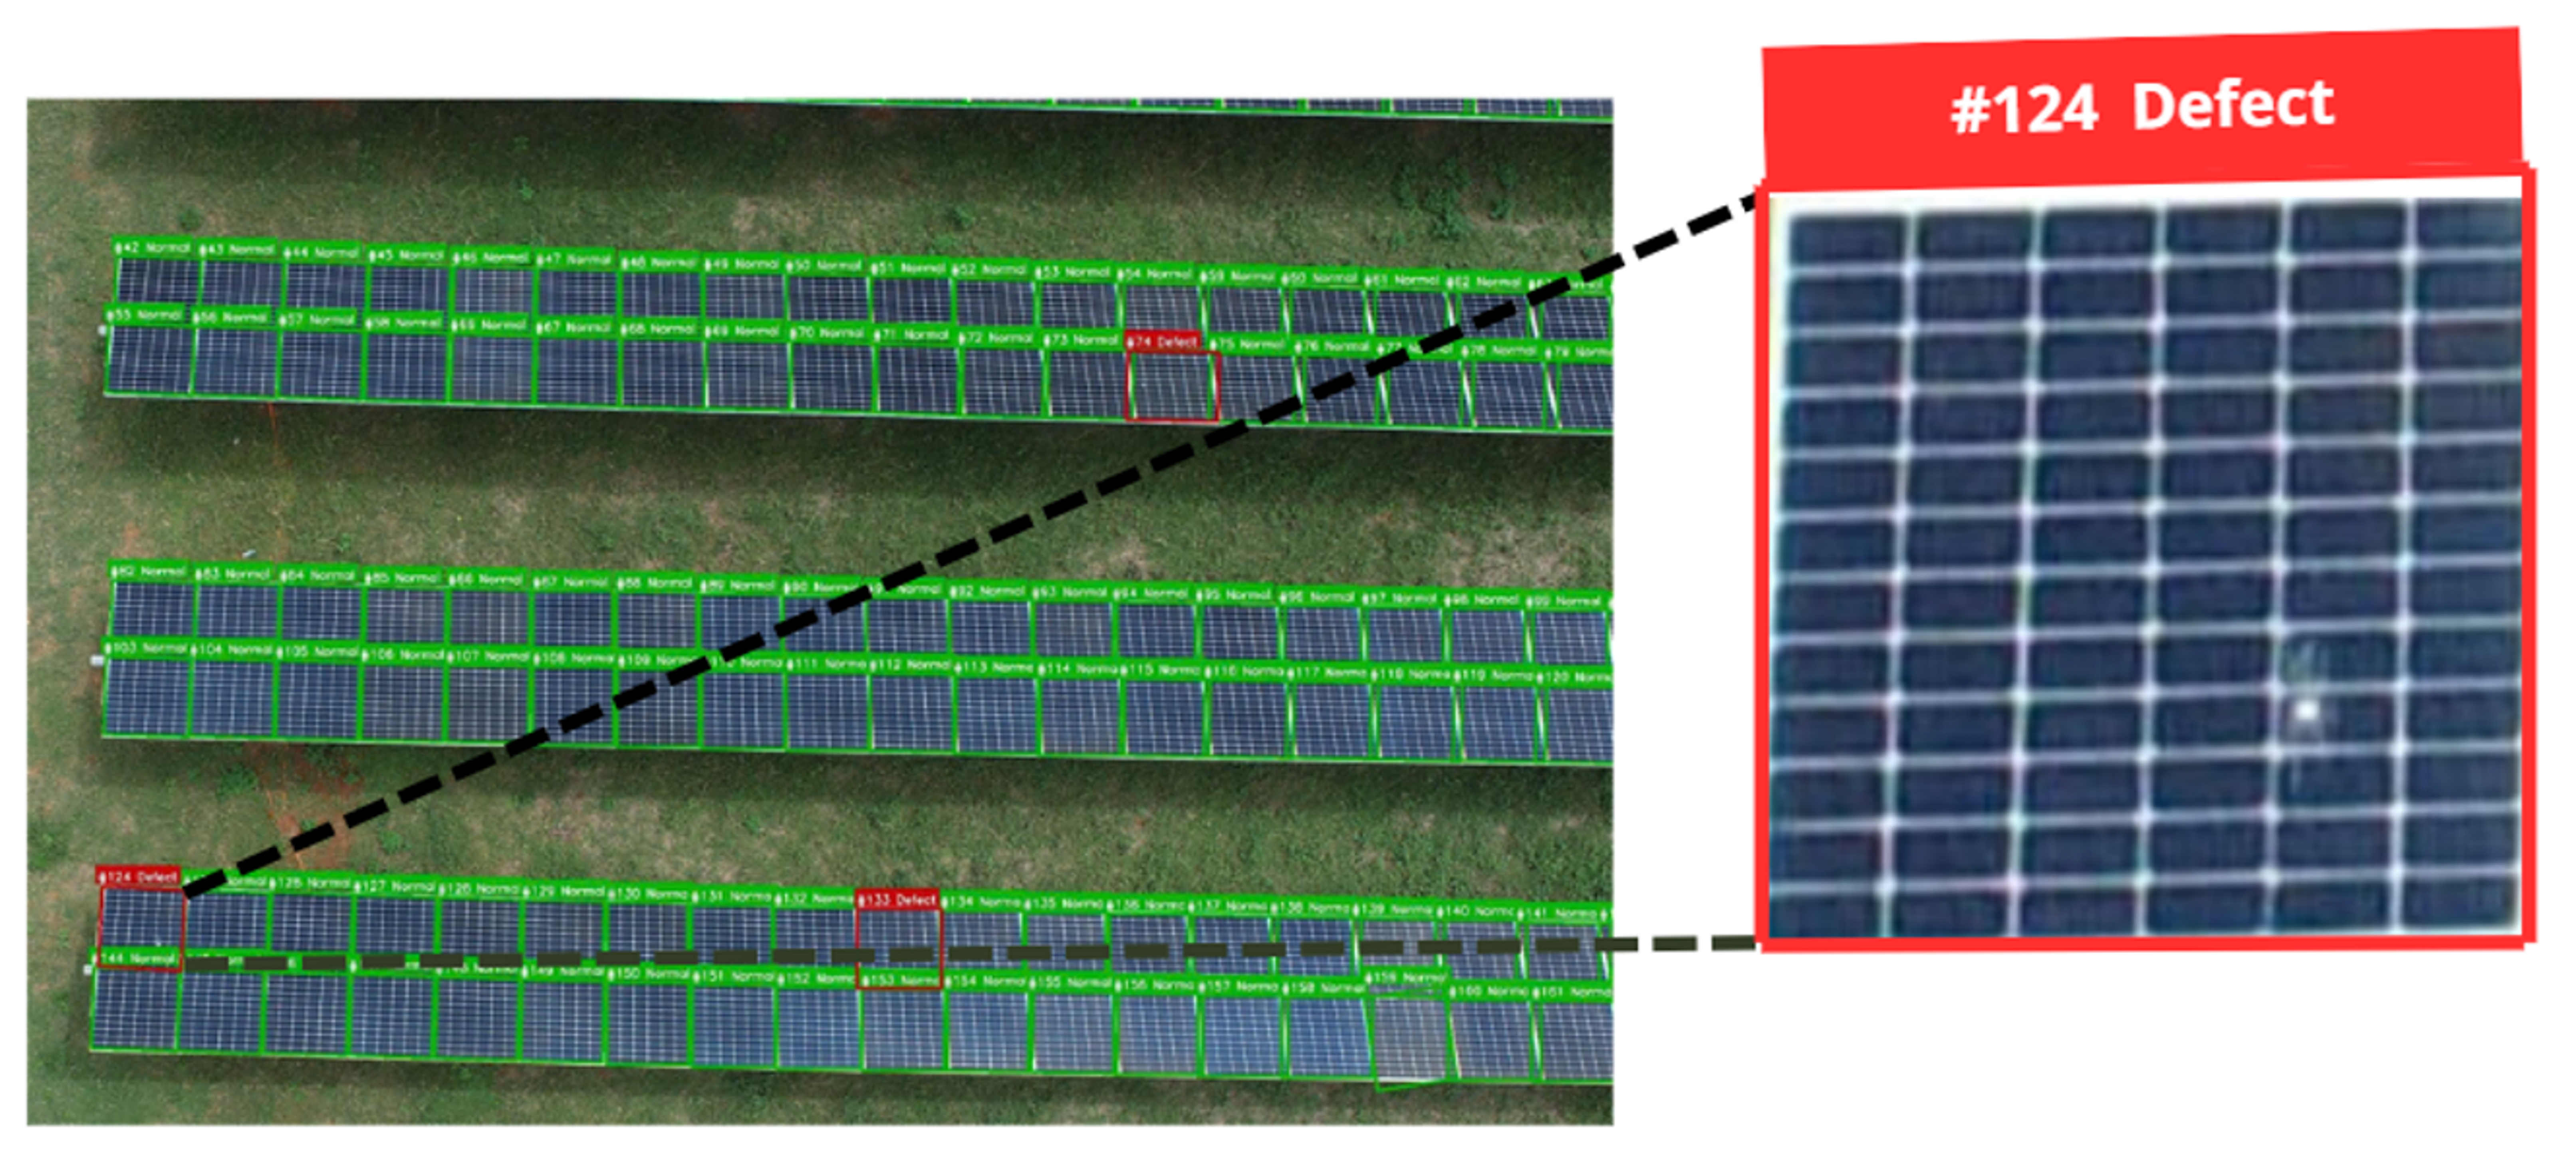
\includegraphics[width=0.8\textwidth]{images/TongKet/demo1.png}
	\end{center}
\end{frame}

% \begin{frame}
% \label{Demo2}
% 	\frametitle{DEMO KẾT QUẢ NHẬN DẠNG}
% 	\begin{center}
% 		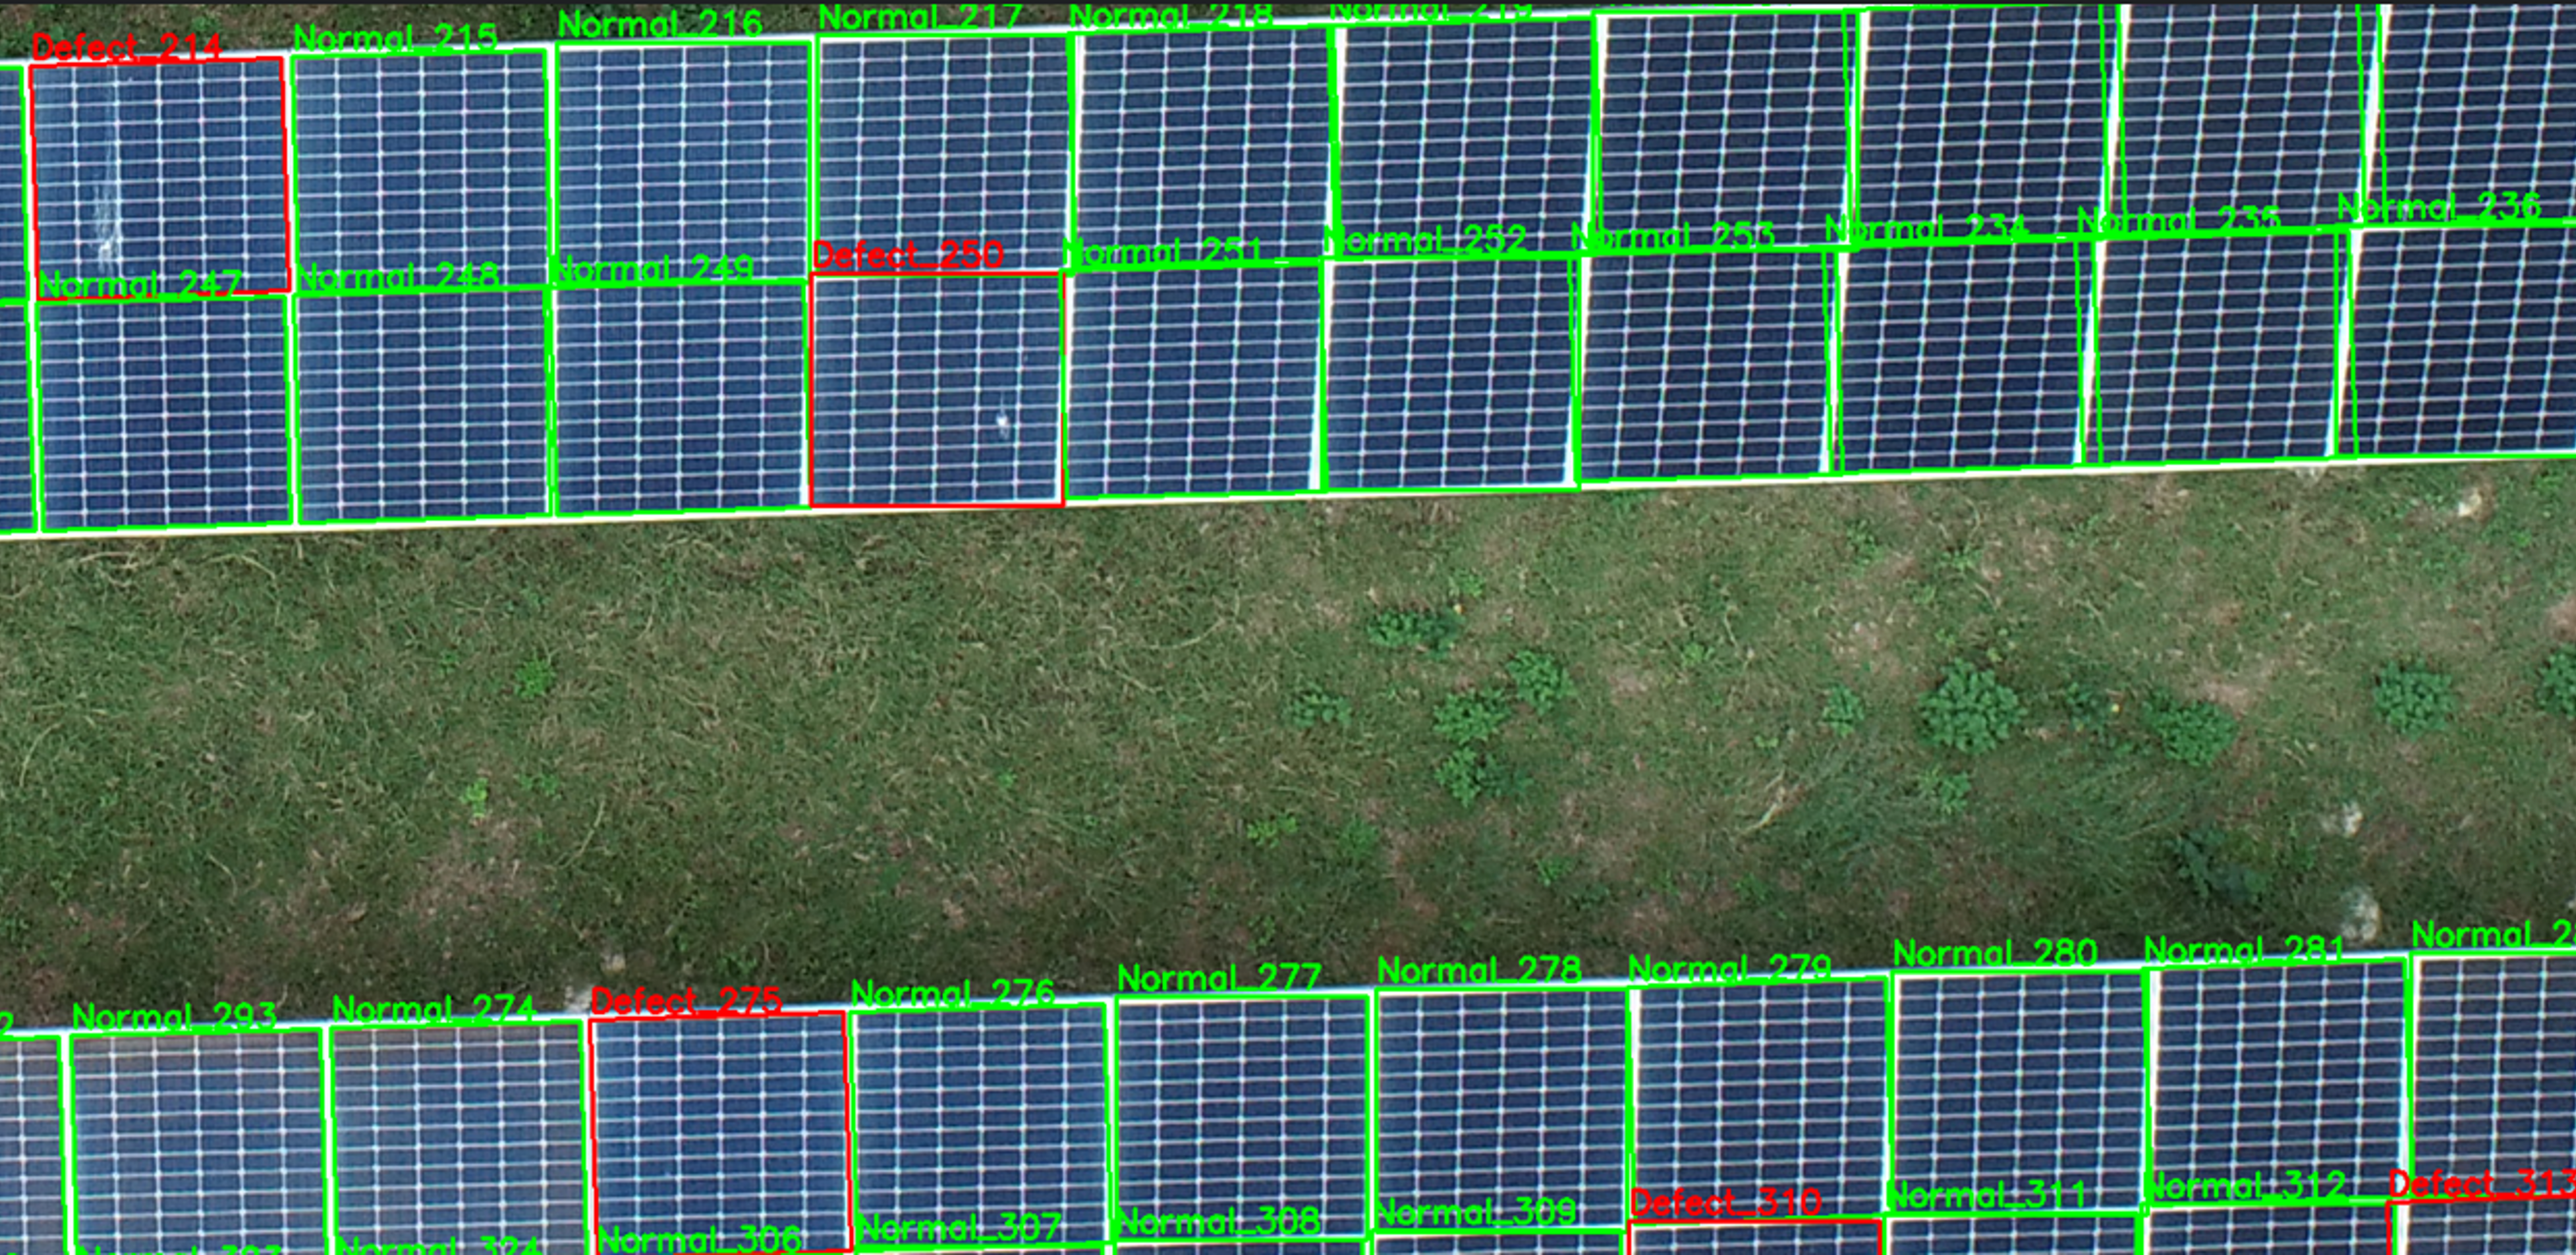
\includegraphics[width=0.8\textwidth]{images/TongKet/demo2.png}
% 	\end{center}
% \end{frame}

\begin{frame}
    \frametitle{SO SÁNH HIỆU SUẤT}
    
    \small 
    \renewcommand{\arraystretch}{1.5}
    \setlength{\tabcolsep}{3pt}
    \setlength{\arrayrulewidth}{1pt} % Tăng độ đậm đường kẻ
    
    \begin{tabularx}{\textwidth}{|>{\centering\arraybackslash\hsize=1.5\hsize}X|*{5}{>{\centering\arraybackslash\hsize=0.9\hsize}X|}}
        \hhline{|-|-|-|-|-|-|}
        \textbf{Mô hình} & \textbf{Accuracy (\%)} & \textbf{Precision} & \textbf{Recall} & \textbf{F1-score} & \textbf{Params (M)} \\
        \hhline{|-|-|-|-|-|-|}
        % Dùng hhline để đường kẻ không bị màu đè
        \rowcolor{highlightYellow} \textbf{EfficientNet-B2} & \textbf{96,45} & \textbf{0,9646} & \textbf{0,9645} & \textbf{0,9645} & \textbf{7,7} \\
        \hhline{|-|-|-|-|-|-|}
        ResNet-34 & 96,25 & 0,9628 & 0,9625 & 0,9625 & 21,29 \\
        \hhline{|-|-|-|-|-|-|}
        ResNet-18 & 95,77 & 0,9585 & 0,9577 & 0,9576 & 11,18 \\
        \hhline{|-|-|-|-|-|-|}
        ResNet-50 & 96,4 & 0,9641 & 0,964 & 0,9639 & 23,51 \\
        \hhline{|-|-|-|-|-|-|}
        VGG16 & 93,57 & 0,9372 & 0,9357 & 0,9356 & 40,94 \\
        \hhline{|-|-|-|-|-|-|}
    \end{tabularx}
    
    \vspace{0.3cm}
    
    \begin{itemize}
        \item \textcolor{red}{\textbf{Nhận Xét:}} EfficientNet-B2 đạt độ chính xác cao nhất (\textbf{96.45\%}).
        \item Mô hình nhẹ hơn gấp \textbf{3 lần} so với ResNet-50 và \textbf{5 lần} so với VGG16.
        \item Thời gian huấn luyện nhanh (~34 phút), phù hợp cho việc tinh chỉnh và cập nhật liên tục.
    \end{itemize}
\end{frame}

\begin{frame}
    \frametitle{KẾT LUẬN}

    \begin{columns}[t] % Căn lề trên để tránh bị lệch dòng
        
        % Cột trái: Kết Quả Đạt Được
        \begin{column}{0.48\textwidth}
            \begin{tcolorbox}[
                colback=orangeBg, 
                colframe=orangeTitle, 
                sharp corners, 
                boxrule=0pt, 
                leftrule=0pt, % Tạo đường kẻ dọc bên trái
                boxsep=2pt,
                left=5pt,
                right=5pt,
                top=5pt,
                bottom=15pt % Tăng khoảng trống dưới để tránh tràn
            ]
                {\color{orangeTitle}\bfseries Kết Quả Đạt Được} \small \vspace{1em}
                \begin{itemize}
                    \item[\color{orangeTitle}\textbf{>}] Xây dựng thành công quy trình tự động: Thu thập $\rightarrow$ Cắt ảnh $\rightarrow$ Phân loại.
                    \item[\color{orangeTitle}\textbf{>}] Thuật toán tách chiết đạt độ chính xác cao (96.9\%).
                    \item[\color{orangeTitle}\textbf{>}] Mô hình AI (EfficientNet-B2) đạt độ chính xác 96.45\%, vượt trội so với các mô hình nền tảng khác.
                \end{itemize}
            \end{tcolorbox}
        \end{column}

        % Cột phải: Ý Nghĩa
        \begin{column}{0.48\textwidth}
            \begin{tcolorbox}[
                colback=blueBg, 
                colframe=blueTitle, 
                sharp corners, 
                boxrule=0pt, 
                leftrule=0pt, 
                boxsep=2pt,
                left=5pt,
                right=5pt,
                top=5pt,
                bottom=38pt % Điều chỉnh để hai hộp cao bằng nhau
            ]
                {\color{blueTitle}\bfseries Ý Nghĩa} \small \vspace{1em}
                \begin{itemize}
                    \item[\color{orangeTitle}\textbf{>}] Chứng minh tính khả thi của việc sử dụng ảnh RGB và CNN hạng nhẹ.
                    \item[\color{orangeTitle}\textbf{>}] Giảm thiểu chi phí và rủi ro cho công tác bảo trì.
                    \item[\color{orangeTitle}\textbf{>}] Nền tảng cho các hệ thống giám sát thời gian thực.
                \end{itemize}
            \end{tcolorbox}
        \end{column}

    \end{columns}
\end{frame}

\begin{frame}
    \frametitle{HẠN CHẾ CỦA ĐỀ TÀI}

    \begin{columns}[t]
        % Cột 1: Phân Loại Nhị Phân
        \begin{column}{0.31\textwidth}
            \begin{tcolorbox}[limitationbox]
                \centering
                \includegraphics[height=0.5cm]{images/TongKet/icons/nhiphan.png} \vspace{0.3cm}
                
                {\color{mainblue}\textbf{Phân Loại Nhị Phân}} \vspace{0.2cm}
                
                Mới chỉ phân biệt được "Lỗi" và "Bình thường". Chưa định danh cụ thể loại lỗi (nứt, bụi, hay che bóng) và chưa định vị tọa độ lỗi trên tấm pin.
            \end{tcolorbox}
        \end{column}

        % Cột 2: Dữ Liệu
        \begin{column}{0.31\textwidth}
            \begin{tcolorbox}[limitationbox]
                \centering
                \includegraphics[height=0.5cm]{images/TongKet/icons/dulieu.png} \vspace{0.3cm}
                
                {\color{mainblue}\textbf{Dữ Liệu}} \vspace{0.2cm}
                
                Tập trung ở một vùng địa lý nhất định. Chưa đa dạng về điều kiện thời tiết, ánh sáng và các kiểu bố trí tấm pin khác nhau.
            \end{tcolorbox}
        \end{column}

        % Cột 3: Giới Hạn RGB
        \begin{column}{0.31\textwidth}
            \begin{tcolorbox}[limitationbox]
                \centering
                \includegraphics[height=0.5cm]{images/TongKet/icons/rgb.png} \vspace{0.3cm}
                
                {\color{mainblue}\textbf{Giới Hạn RGB}} \vspace{0.2cm}
                
                Không phát hiện được các lỗi nhiệt (Hotspot) hoặc lỗi bên trong tế bào (Cell defects) nếu không có biểu hiện ra bề mặt.
            \end{tcolorbox}
        \end{column}
    \end{columns}
\end{frame}

% Cấu hình khung tcolorbox cho giống mẫu
\newtcolorbox{featurebox}{
    colback=white,
    colframe=gray!30,
    arc=5pt,
    boxrule=0.5pt,
    valign=top,
    halign=center,
    height=5.5cm, % Cố định chiều cao để các hộp bằng nhau
    width=\textwidth
}

\begin{frame}
    \frametitle{HƯỚNG PHÁT TRIỂN TIẾP THEO}
    
    \begin{columns}[t, onlytextwidth]
        
        % Cột 1: Đa Phương Thức
        \begin{column}{0.31\textwidth}
            \begin{featurebox}
                \includegraphics[height=1cm]{images/TongKet/icons/multimodal.png} \vspace{0.3cm}
                
                \textbf{\small Đa Phương Thức (Multimodal)} \vspace{0.2cm}
                
                \scriptsize Kết hợp ảnh nhiệt (Thermal) để phát hiện các lỗi vô hình như Hotspots, PID bên trong cell.
            \end{featurebox}
        \end{column}
        
        % Cột 2: Định Vị Tấm Pin Lỗi
        \begin{column}{0.31\textwidth}
            \begin{featurebox}
                \includegraphics[height=1cm]{images/TongKet/icons/dinhvi.png} \vspace{0.3cm}
                
                \textbf{\small Định Vị Tấm Pin Lỗi} \vspace{0.2cm}
                
                \scriptsize Kết hợp tọa độ pixel của tấm pin với GPS/RTK và layout nhà máy để ánh xạ đúng vị trí thực tế, giúp kỹ thuật viên xác định nhanh điểm cần kiểm tra.
            \end{featurebox}
        \end{column}
        
        % Cột 3: Định Vị & Phân Đoạn
        \begin{column}{0.31\textwidth}
            \begin{featurebox}
                \includegraphics[height=1cm]{images/TongKet/icons/phandoan.png} \vspace{0.3cm}
                
                \textbf{\small Định Vị \& Phân Đoạn} \vspace{0.2cm}
                
                \scriptsize Chuyển từ Phân loại (Classification) sang Phát hiện đối tượng (YOLO) để khoanh vùng chính xác vị trí lỗi.
            \end{featurebox}
        \end{column}
        
    \end{columns}
\end{frame}

%------------------------------------------------
% SLIDE PHỤ LỤC 1
\begin{frame}
    \frametitle{PHỤ LỤC}
    \vspace{-0.2cm} % Điều chỉnh khoảng cách để tối đa không gian
    \begin{columns}[c, onlytextwidth]
        % --- CỘT TRÁI ---
        \begin{column}{0.48\textwidth}
            \centering
            % Ảnh được căn giữa và co giãn tối đa nhưng không vượt quá kích thước cột và slide
            \includegraphics[width=\linewidth, height=0.8\textheight, keepaspectratio]{images/PhuLuc/1.jpg}
        \end{column}

        % --- CỘT PHẢI ---
        \begin{column}{0.48\textwidth}
            \centering
            % Ảnh bên phải cũng tương tự
            \includegraphics[width=\linewidth, height=0.9\textheight, keepaspectratio]{images/PhuLuc/3.png}
        \end{column}
    \end{columns}
\end{frame}

%------------------------------------------------
% SLIDE PHỤ LỤC 2
\begin{frame}
    \frametitle{PHỤ LỤC}
    \begin{center}
        \includegraphics[width=1\textwidth, height=0.82\textheight, keepaspectratio]{images/PhuLuc/2.png}
    \end{center}
\end{frame}